\section{Results}


%Presents the results of the procedure and includes:
%1) all data collected in tabular form if possible;
%2) all required graphs;
%3) all results in a logical sequence;
%4) objective observations;
%Note: all figures, tables and graphs required should include
%titles, labels, units and legends where appropriate.

%Present processed data, not raw data.

%The accepted value of $\gamma$ for dry air at room temperature ($\gamma = 1.40$) was taken from standard reference
%data~\cite{CRC}.

\begin{figure}[htb]
    \centering
    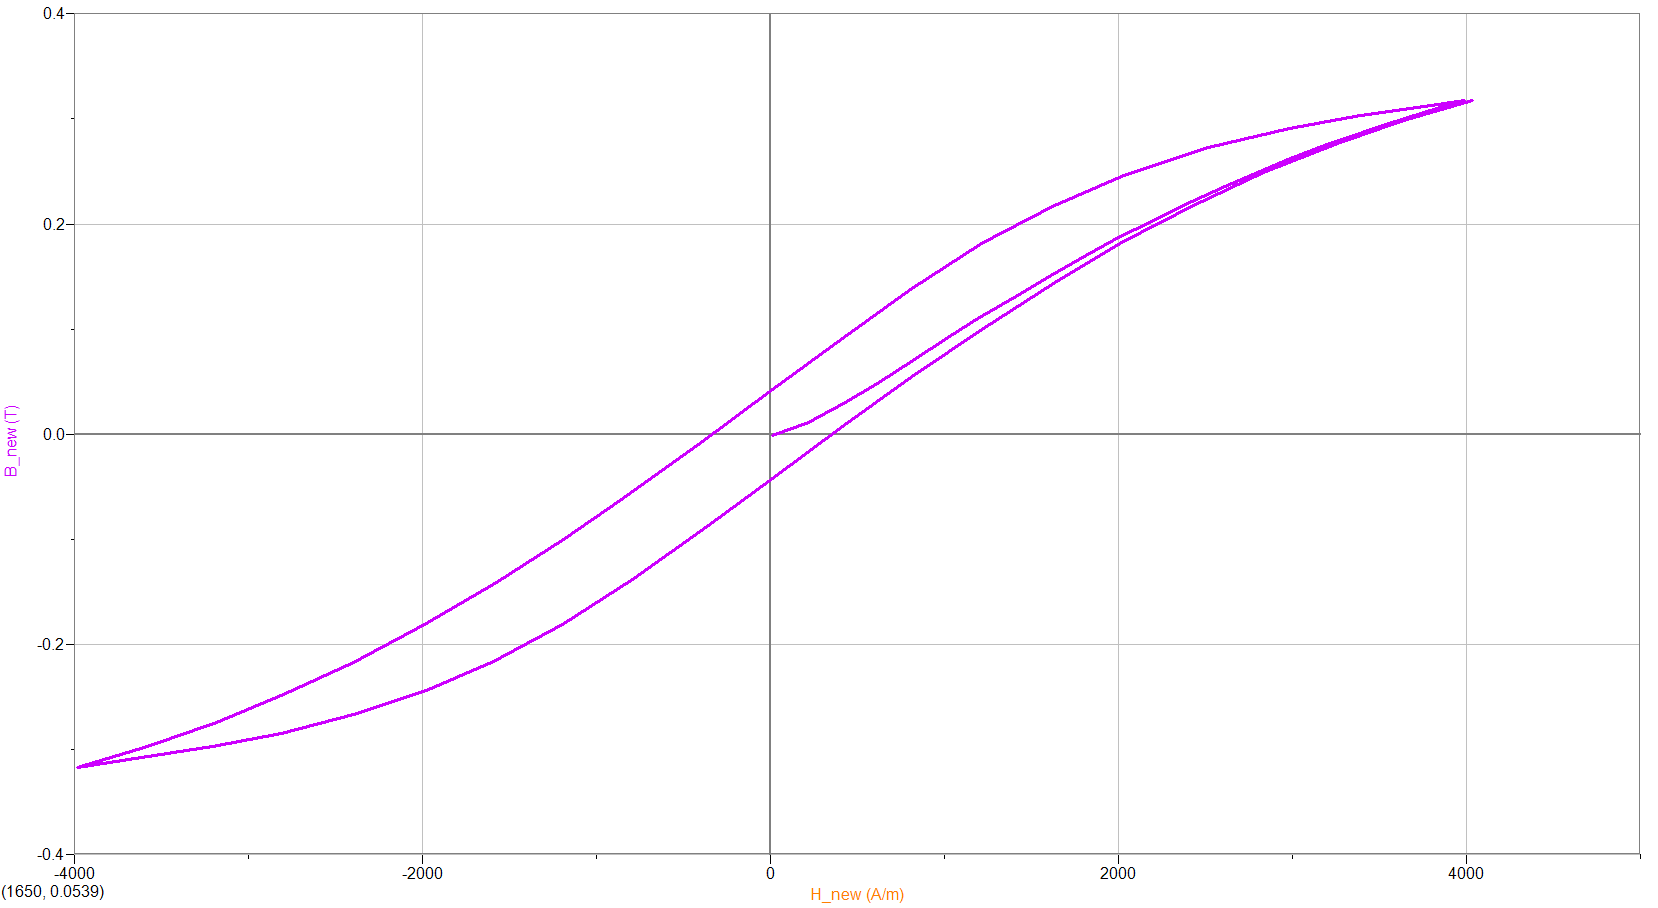
\includegraphics[width=\linewidth]{figs/hysteresis}
    \caption
    {The full magnetic response of the material from -2.0 A to + 2.0 A. The y-axis is $\vec{B}$, x-axis is $\vec{H}$}
    \label{fig:hysteresis}
\end{figure}

Figure~\ref{fig:hysteresis} shows the full data captured from the experiment.
The magnetic response was different depending on whether forward or reverse current was applied, and the which
direction it was incremented (towards 2.0 Amps or zero).

\begin{figure}[htb]
    \centering
    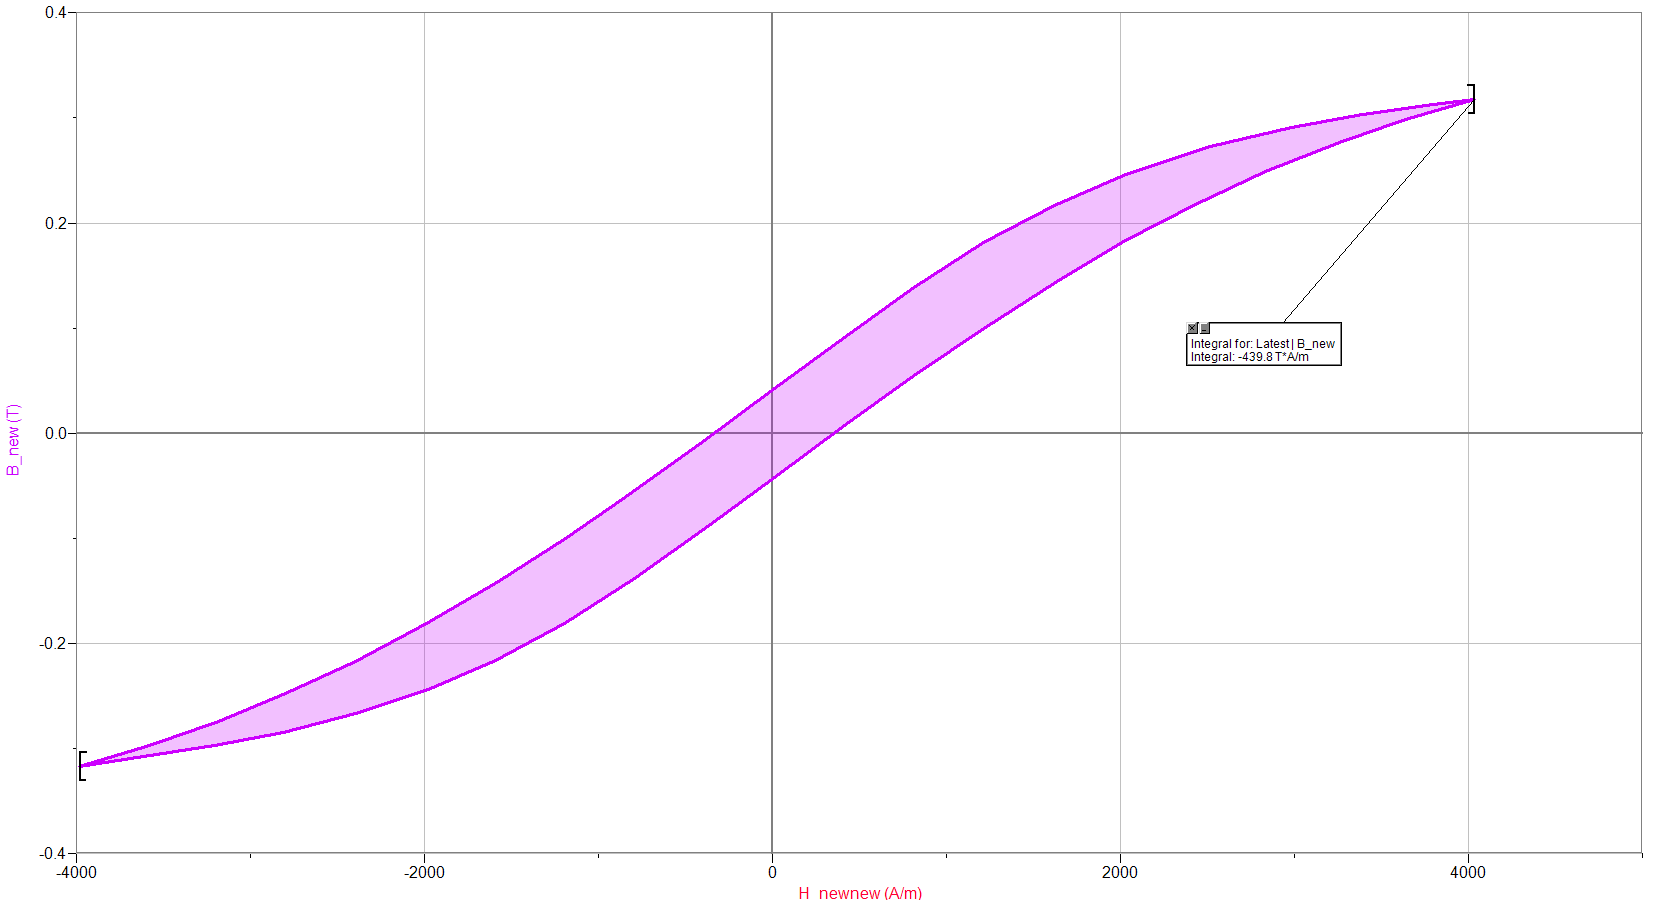
\includegraphics[width=\linewidth]{figs/integral}
    \caption{The integral of the closed loop was done with the LoggerPro software, minus the initial phase. Area
        = -439.8 T A/m.}
    \label{fig:integral}
\end{figure}

Integrating the closed loop as shown in Figure~\ref{fig:integral} produced an area of \qty{439.8}{\tesla\ampere\per\meter}.
From Eq.~\eqref{eq:work}, the area of enclosed by the curve is equal to the work done per volume.
The units from the plot are \qty{}{\tesla\ampere\per\meter}.
This is equivalent to \qty{}{\meter\kilogram\second} by performing dimensional analysis:

%\begin{align*}
%    \frac{\unit{\tesla\ampere}}{\unit{\meter}} &= \frac{\unit{\newton}}{\unit{\ampere\meter}}
%    \frac{\unit{\ampere}}{\unit{
%        \meter}} \\
%    &= \frac{\unit{\newton}}{\meter^2} \\
%    &= \frac{\unit{\newton\meter}}{\unit{\meter^3}} \\
%    &= \frac{\unit{\joule}}{\unit{\meter^3}} \quad \because \unit{\joule} = \unit{\newton\meter}
%\end{align*}


\begin{align*}
    \frac{\unit{\tesla\ampere}}{\unit{\meter}}
      &= \frac{\unit{\newton}}{\unit{\ampere\meter}}
         \cdot \frac{\unit{\ampere}}{\unit{\meter}} \\
      &= \frac{\unit{\newton}}{\unit{\meter\squared}} \\
      &= \frac{\unit{\newton\meter}}{\unit{\meter\cubed}} \\
      &= \frac{\unit{\joule}}{\unit{\meter\cubed}}
         && \because \unit{\joule} = \unit{\newton\meter}
\end{align*}


Now this can be expressed in meter-kilogram-second units.

\begin{align*}
    \frac{\unit{\joule}}{\unit{\meter}^3} &= \unit{\kilogram} \frac{\unit{\meter}^2}{\unit{\second}^2}
    \frac{1}{\unit{\meter}^3} \\
    &= \frac{\unit{\kilogram}}{\unit{\meter\second^2}}
\end{align*}

The value is unchanged, so this can be represented as \qty{439.8}{\kilogram\per\meter\second^2}.
This area represents the work done per unit volume by the current to magnetise the material throughout the whole
cycle.

The specific heat capacity of steel is \qty{420}{\joule\per\kilogram\per\celsius}.
Using the density of steel, \qty{7.8E3}{\kilogram\per\meter^3} we determine the temperature increase due the work done
throughout the whole cycle we perform the following
calculation:

\begin{align*}
    c &= \frac{W}{m \Delta T} \quad \text{specific heat}\\
    \implies \Delta T &= \frac{W}{V} \frac{1}{\rho c} \\
    &= (439.8) \frac{1}{(\qty{7.8E3}{}) (420)} \unit{\celsius} \\
    &= \qty{1.34E-4}{\celsius}
\end{align*}

\qty{1.34E-4}{\celsius} is the temperature increase if we assume all the work done is converted into Joule heating in the steel.
Since this is less than a tenth of a degree Celsius, this temperature increase would not be directly measurable
using a thermometer with a \qty{0.1}{\celsius} resolution.
Practical uses of measuring this temperature would be to protect sensitive electronic equipment.
Any measurable increase in temperature would indicate a large, perhaps unexpected current surge.
Alternatively, since heat accumulates, a noticeable temperature increase would give an
indication that the material had undergone multiple cycles.

\begin{figure}[htb]
    \centering
    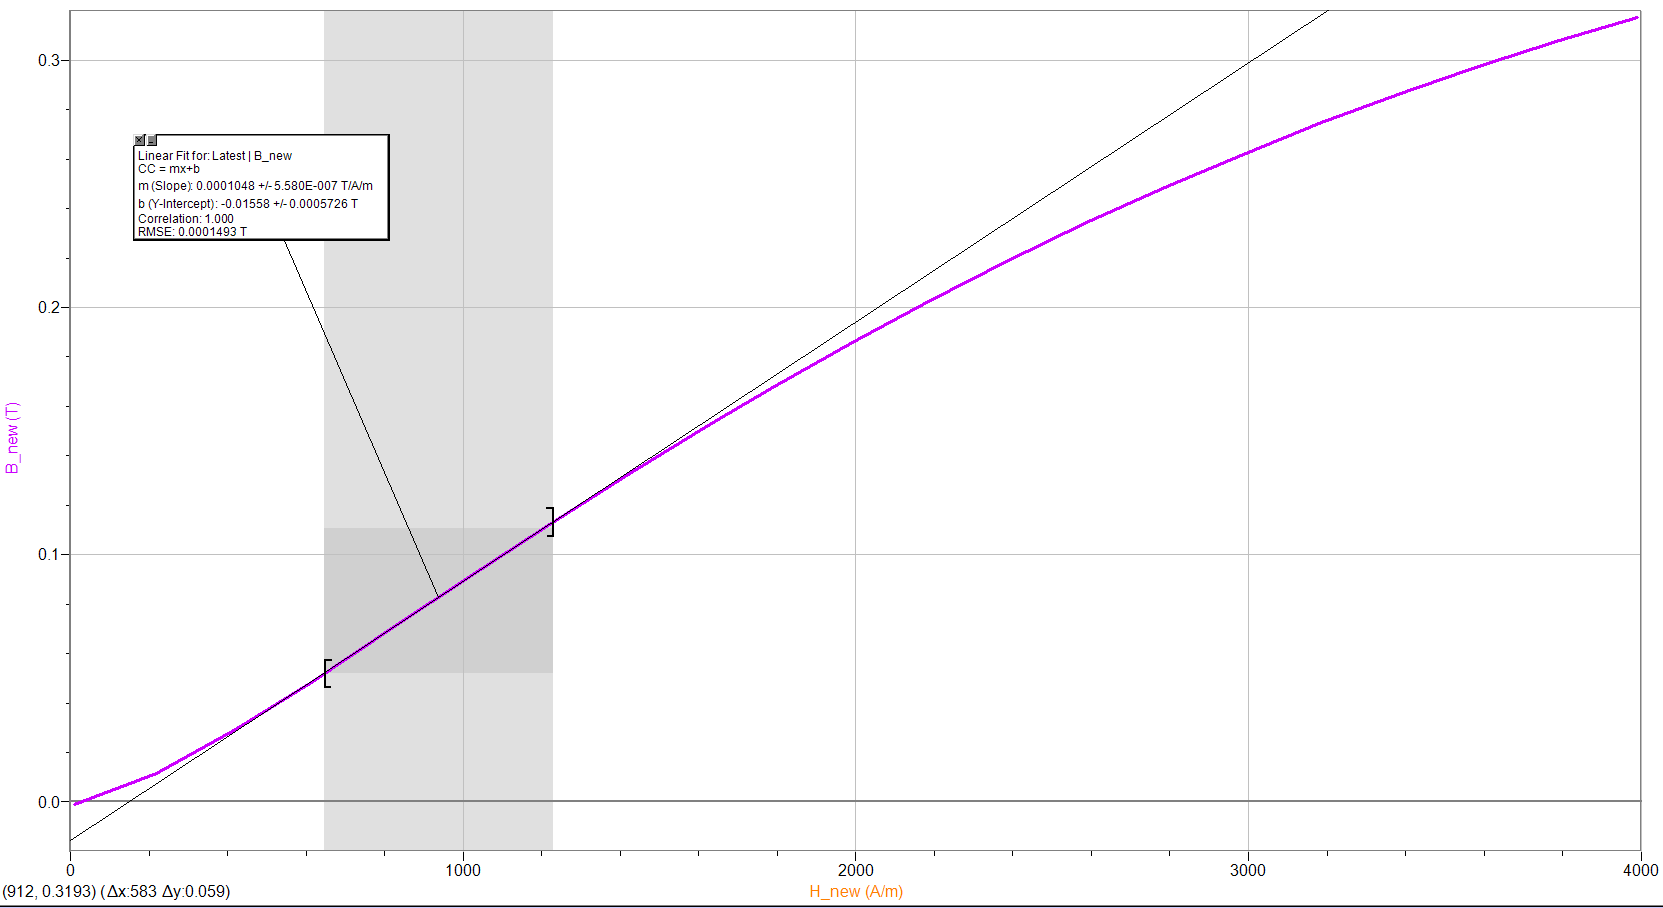
\includegraphics[width=\linewidth]{figs/slope}
    \caption{The maximum slope found during the initial phase. Slope =
    $\qty{104.8(0.56)e-6}{\tesla\meter\per\ampere}$}\label{fig:slope}
\end{figure}

By examining the maximum slope of the initial phase as in Figure~\ref{fig:slope}, we can determine the maximum susceptibility of
the
material via
Eq.~\eqref{eq:chi}.

\begin{align*}
    B &= \mu_0(1 + \chi) H \\
    \implies \chi &= \frac{B}{\mu_0 H} - 1 \\
    &= \frac{\qty{104.80(0.56)E-6}{}}{(4 \pi \times 10^{-7})} - 1 \\
    &= \qty{82.40(0.45)}{}
\end{align*}

This value, magnetic susceptibility, represents how strongly the material aligns with the applied magnetic field.
Since this was derived from the maximum slope, this is the maximum susceptibility of the material.




%\begin{table}[htbp]
%    \caption{Final results}
%    \resizebox{\columnwidth}{!}{%
%        \begin{tabular}{llccc}
%            \toprule
%            Gas                 & Experimental  & Accepted & Error (\%) & Consistency \\
%            \midrule
%            Air                 & 1.369+/-0.064 & 1.402    & 2.35       & PASS        \\
%            Argon               & 1.625+/-0.076 & 1.664    & 2.37       & PASS        \\
%            CO\textsubscript{2} & 1.278+/-0.060 & 1.293    & 1.15       & PASS        \\
%            \bottomrule
%        \end{tabular}
%    }
%    \label{tab:results}
%\end{table}

% Transposed version
%\begin{table}[htbp]
%    \caption{Final results}
%    \centering
%    \begin{tabular}{lr}
%        \toprule
%        Quantity     & $\mu_B$                              \\
%        \midrule
%        Experimental & \qty{8.3(0.4)e-24}{\joule\per\tesla} \\
%        Accepted     & \qty{0.9273e-23}{\joule\per\tesla}   \\
%        Error (\%)   & 11                                   \\
%        Consistency  & FAIL                                 \\
%        \bottomrule
%    \end{tabular}
%    \label{tab:results2}
%\end{table}


%\textcolor{red}{
%    Uncertainties in experimental values were calculated using the aid of the \textit{uncertainties} python package.
%}
